\addcontentsline{toc}{section}{APPENDICES}	% Add appendices section to toc
\section*{APPENDICES} 						% Section name

\subsection*{A} 
\label{appendix:schematic}
%
\begin{figure}[H]
    \centering
    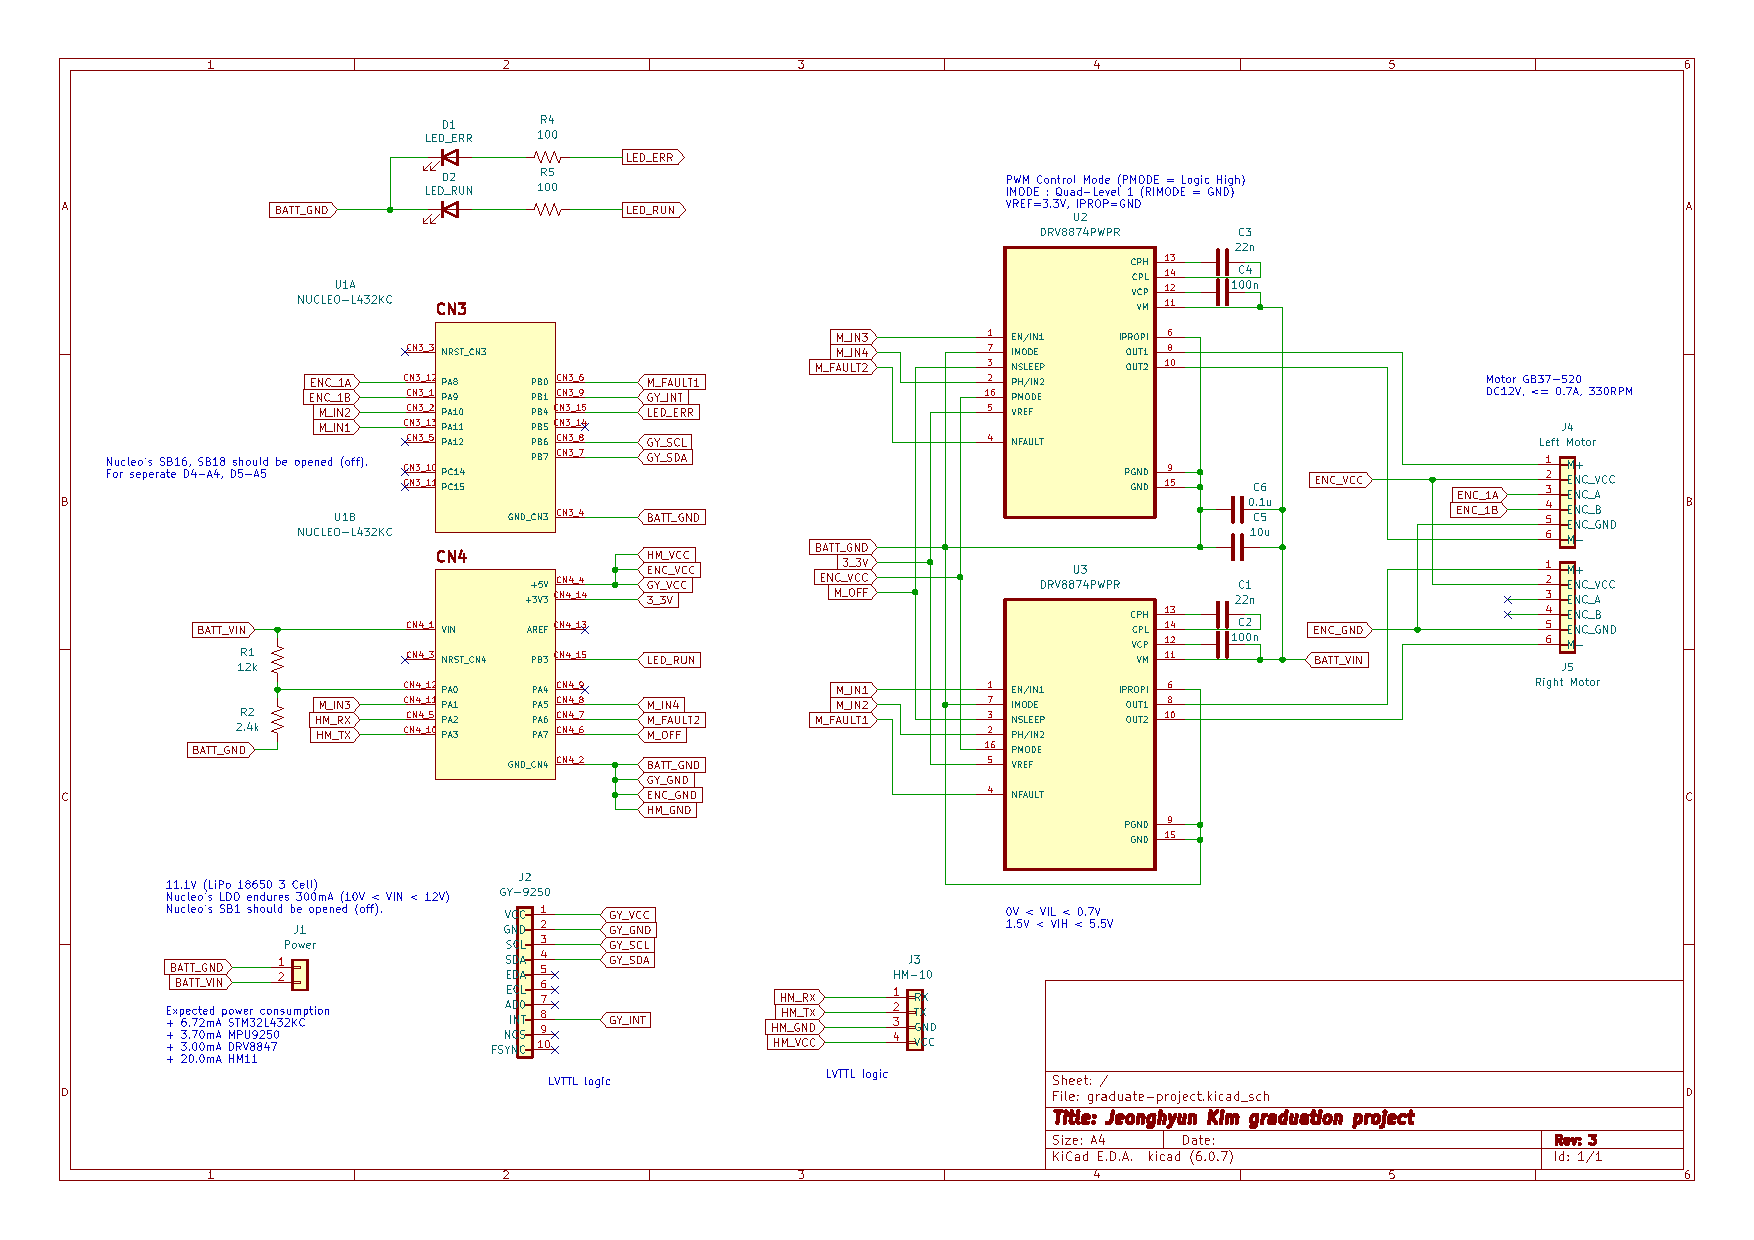
\includegraphics[width=\textwidth]{figures/circuit.pdf}
    \label{fig:schematic}
\end{figure}
%
\subsection*{B}
\label{appendix:gerber}
%
\begin{figure}[H]
\centering
\subfloat[Front]{
    \centering
    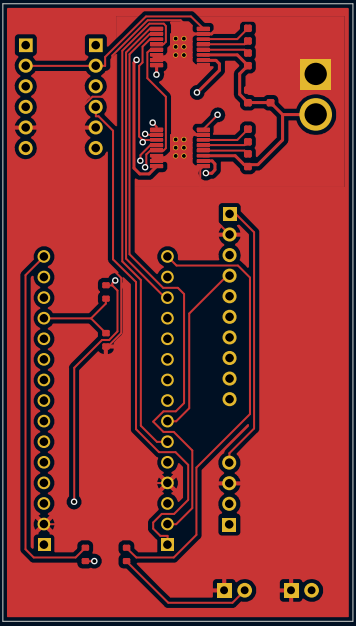
\includegraphics[width=0.2\textwidth]{figures/pcb_front.PNG}
    \label{fig:pcb_front}
}
\subfloat[Back]{
    \centering
    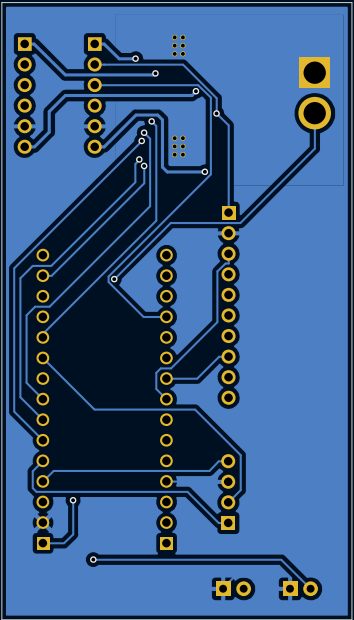
\includegraphics[width=0.2\textwidth]{figures/pcb_back.PNG}
    \label{fig:pcb_back}
}
\subfloat[Assembly]{
    \centering
    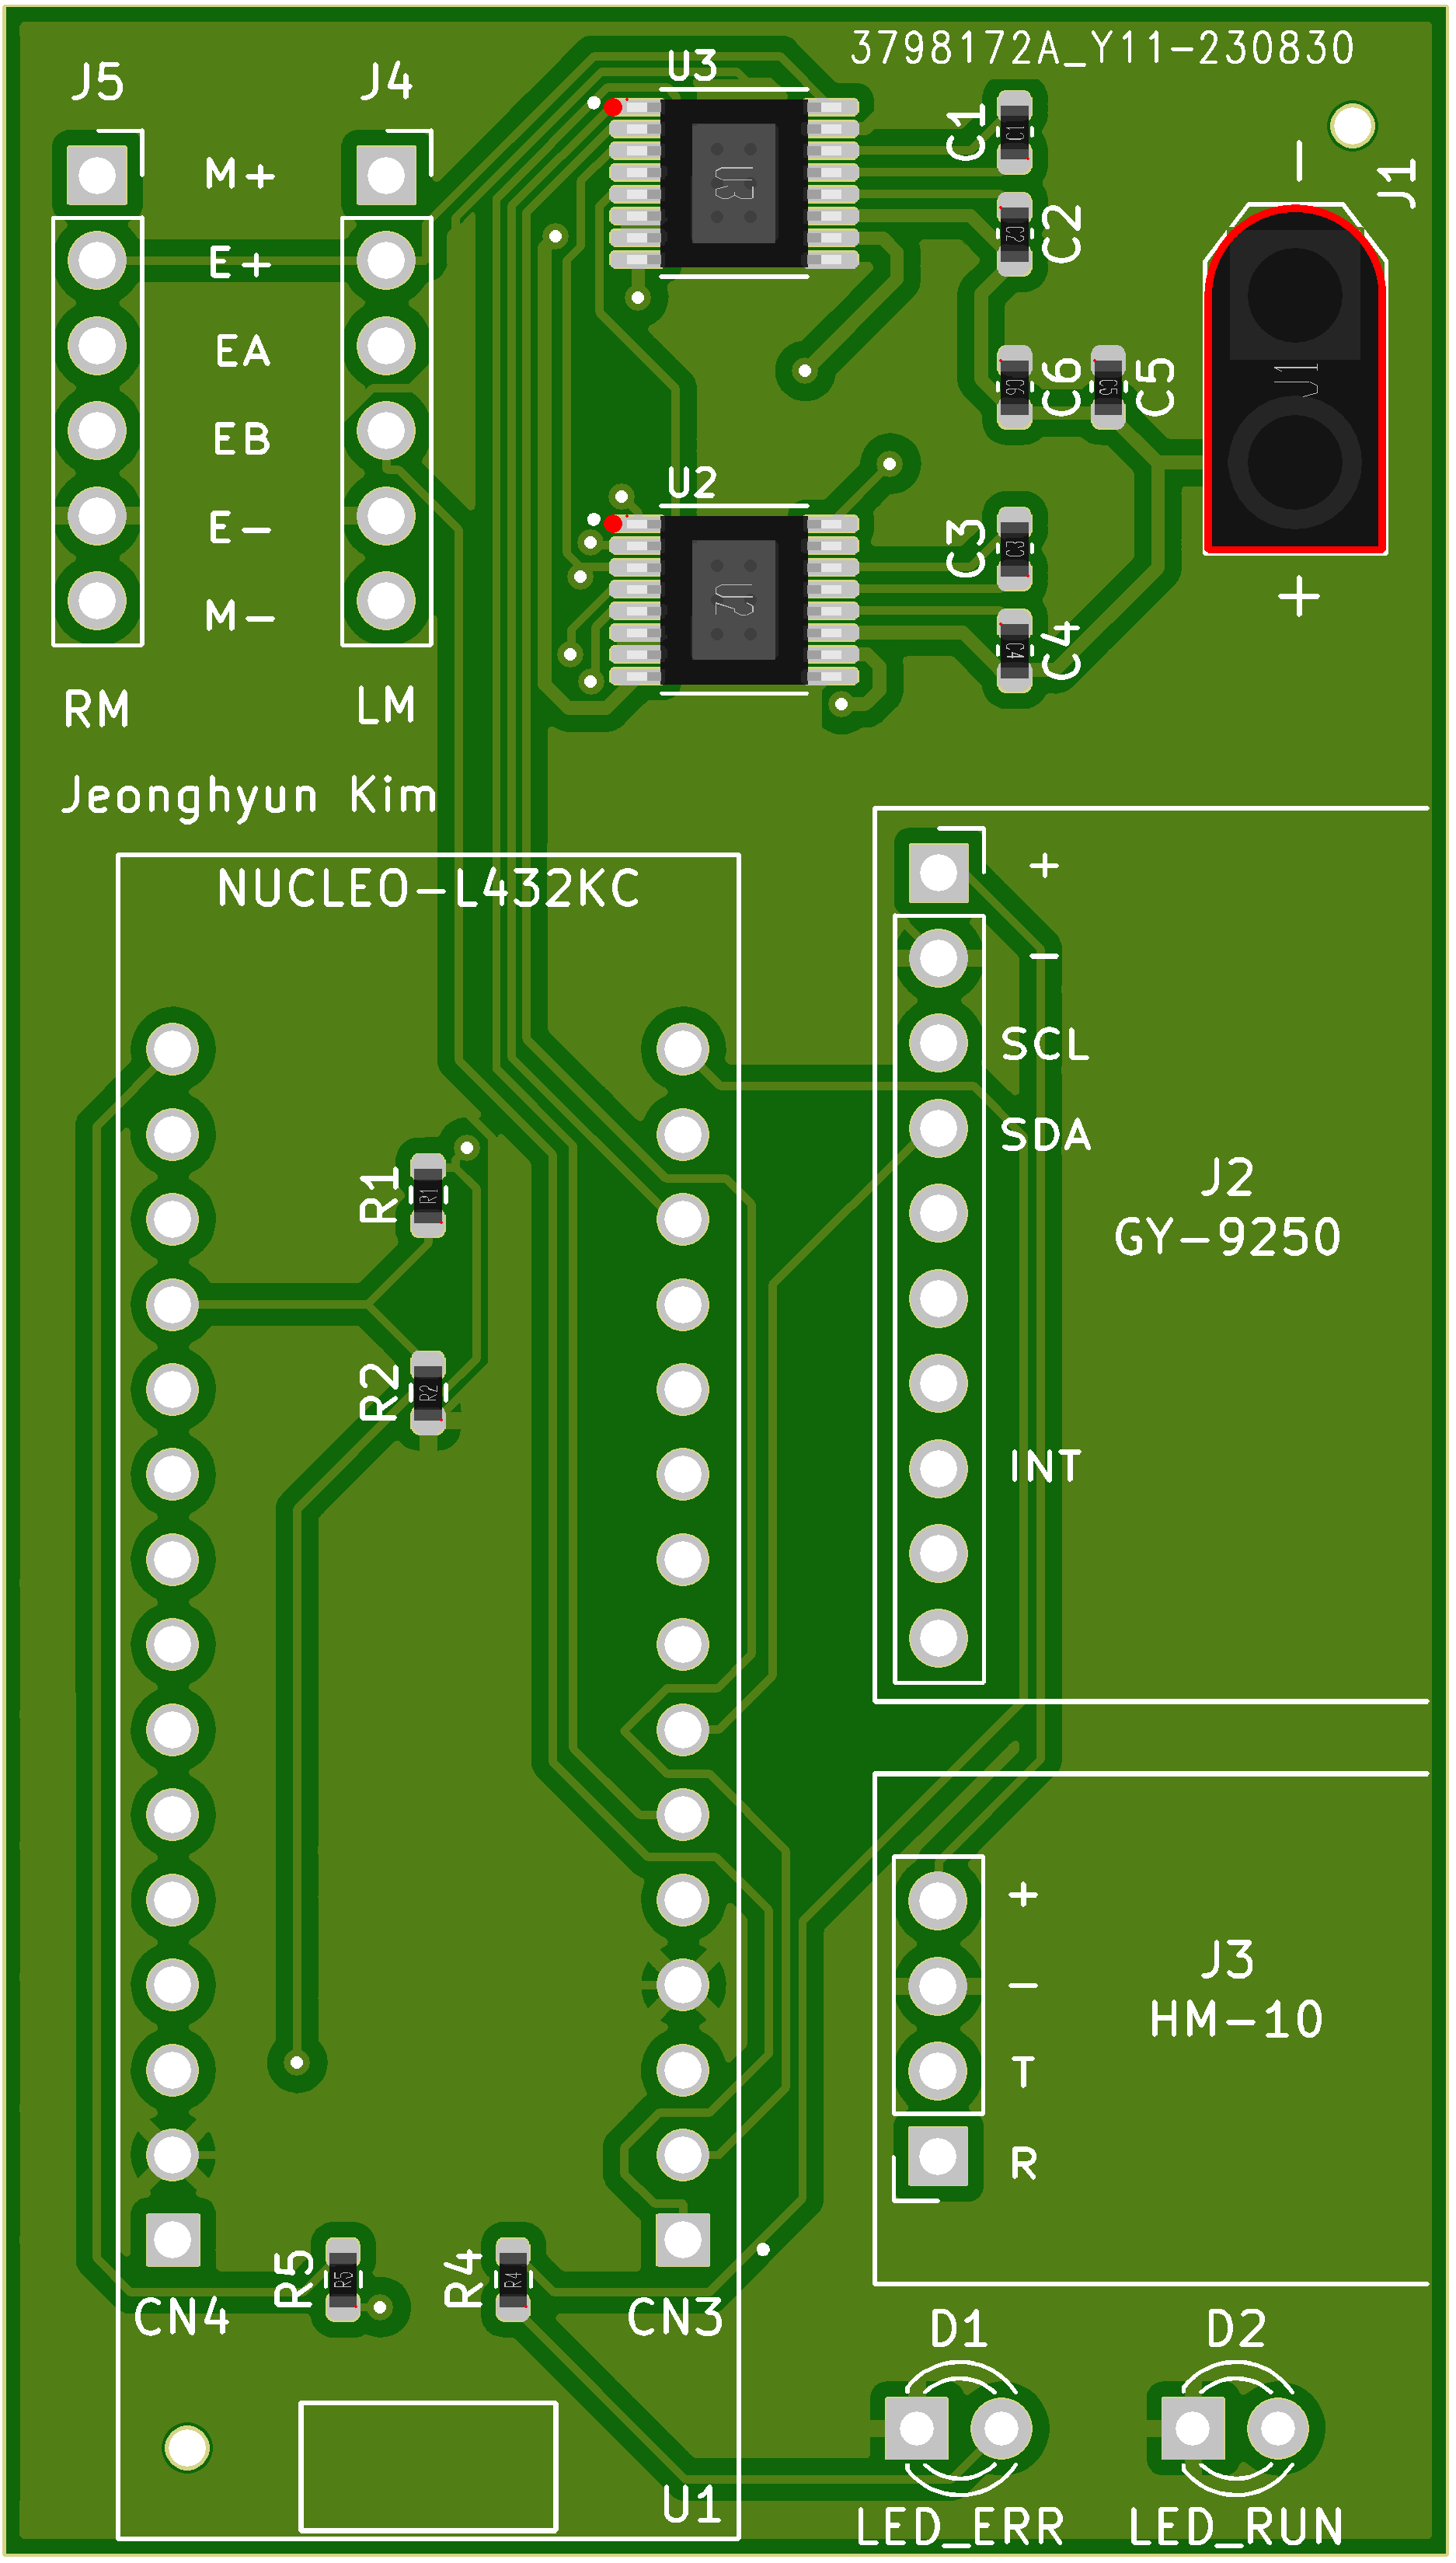
\includegraphics[width=0.2\textwidth]{figures/pcb_assy.png}
    \label{fig:pcb_assy}
}
\end{figure}
%
\subsection*{C}
\label{appendix:source}
구현된 소스 코드는 아래 Github 저장소에서 확인할 수 있습니다.
\begin{itemize}
    \item 시뮬레이션 및 소프트웨어 : \\ \url{https://github.com/Dictor/RBFPID-Balbot-firmware/}
    \item 텔레메트리 소프트웨어 : \\ \url{https://github.com/Dictor/RBFPID-Balbot-telemetry/}
    \item 회로도 및 PCB 거버 : \\ \url{https://github.com/Dictor/RBFPID-Balbot-circuit/}
\end{itemize}
%